\documentclass[a4paper,12pt]{article}
\usepackage{fontspec}
\setmainfont{Noto Serif CJK JP}[Scale=1.0]
\usepackage{amsmath,amssymb,amsthm}
\usepackage{tikz-cd}
\usepackage{tikz}
\usetikzlibrary{positioning,shapes,arrows}
\usepackage{hyperref}
\usepackage[margin=25mm]{geometry}

\theoremstyle{definition}
\newtheorem{definition}{定義}[section]
\newtheorem{theorem}[definition]{定理}
\newtheorem{lemma}[definition]{補題}
\newtheorem{proposition}[definition]{命題}
\newtheorem{example}[definition]{例}
\newtheorem{remark}[definition]{注意}

\title{Bourbaki流構造塔の数学的解説}
\author{Claude (Anthropic) によるTeX生成\\CODEX (OpenAI) によるLean形式化}
\date{\today}

\begin{document}

\maketitle

\begin{abstract}
本稿では、Nicolas Bourbakiの集合論的アプローチに基づく「構造塔」(Structure Tower)の概念を学部生向けに解説する。構造塔は、前順序集合によって添字付けられた集合の族であり、順序関係に従って単調に増大する性質を持つ。本稿では、Lean 4による形式化コードを基に、その数学的背景と主要な性質を詳しく説明する。
\end{abstract}

\tableofcontents

\section{導入}

\subsection{Bourbakiの数学的構造}

Nicolas Bourbaki(ブルバキ)は、20世紀の数学を体系化したフランスの数学者集団の筆名である。彼らは数学を「構造」の観点から統一的に記述することを試みた。その中核となる考え方は、集合に様々な「構造」を載せることで、代数的構造(群、環、体など)、順序構造、位相構造といった数学的対象を統一的に扱うというものである。

\subsection{構造塔の動機}

数学において、しばしば複数のレベルにわたって構造を積み上げていく状況に遭遇する。例えば:
\begin{itemize}
\item 数体系の拡大: $\mathbb{N} \subseteq \mathbb{Z} \subseteq \mathbb{Q} \subseteq \mathbb{R} \subseteq \mathbb{C}$
\item 位相空間の細分: より細かい位相からより粗い位相への移行
\item 代数系の拡大: 部分構造から全体構造への包含
\end{itemize}

このような階層的な構造を形式化するのが「構造塔」である。

\section{数学的定義}

\begin{definition}[前順序集合]
集合$\iota$上の二項関係$\leq$が\textbf{前順序}(preorder)であるとは、以下の2つの性質を満たすことをいう:
\begin{enumerate}
\item 反射律: 任意の$i \in \iota$に対して$i \leq i$
\item 推移律: $i \leq j$かつ$j \leq k$ならば$i \leq k$
\end{enumerate}
前順序集合は反対称律(つまり$i \leq j$かつ$j \leq i$ならば$i = j$)を要求しないため、順序集合より一般的である。
\end{definition}

\begin{definition}[構造塔]\label{def:tower}
$\iota$を前順序集合、$\alpha$を型(集合)とする。\textbf{構造塔}(Structure Tower)$T : \text{StructureTower}(\iota, \alpha)$とは、以下のデータからなる:
\begin{enumerate}
\item 各添字$i \in \iota$に対して、$\alpha$の部分集合$T.\text{level}(i) \subseteq \alpha$
\item 単調性条件: 任意の$i, j \in \iota$に対して、$i \leq j$ならば$T.\text{level}(i) \subseteq T.\text{level}(j)$
\end{enumerate}
\end{definition}

\begin{remark}
Leanコードでは、これは次のように定義される:
\begin{verbatim}
structure StructureTower (ι α : Type*) [Preorder ι] : Type _ where
  level : ι → Set α
  monotone_level : ∀ {i j}, i ≤ j → level i ⊆ level j
\end{verbatim}
\end{remark}

\subsection{視覚的理解}

構造塔を視覚的に表現すると以下のようになる:

\begin{center}
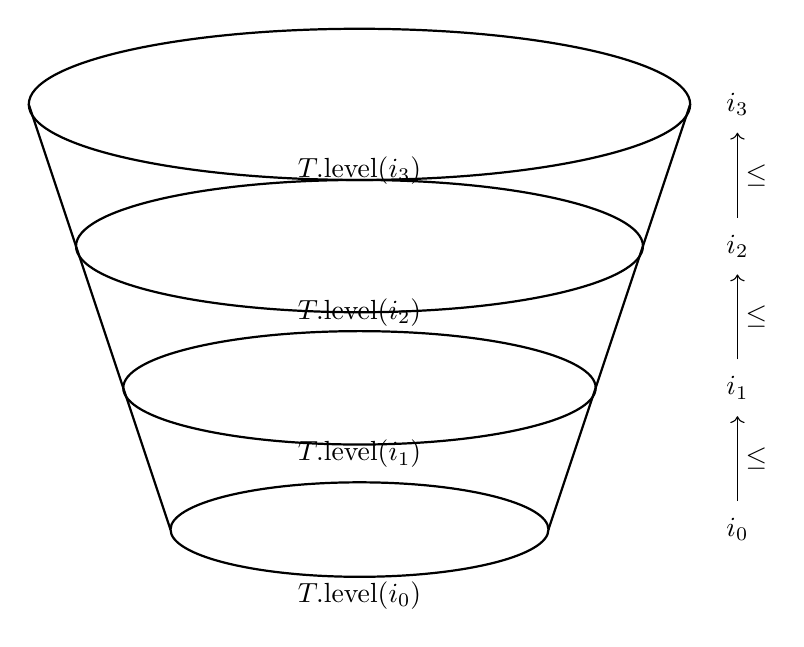
\begin{tikzpicture}[scale=1.2]
% 底面
\draw[thick] (0,0) ellipse (2 and 0.5);
\node at (0,-0.7) {$T.\text{level}(i_0)$};

% 中間層
\draw[thick] (0,1.5) ellipse (2.5 and 0.6);
\node at (0,0.8) {$T.\text{level}(i_1)$};

% 上層
\draw[thick] (0,3) ellipse (3 and 0.7);
\node at (0,2.3) {$T.\text{level}(i_2)$};

% 頂上
\draw[thick] (0,4.5) ellipse (3.5 and 0.8);
\node at (0,3.8) {$T.\text{level}(i_3)$};

% 側面の線
\draw[thick] (-2,0) -- (-2.5,1.5) -- (-3,3) -- (-3.5,4.5);
\draw[thick] (2,0) -- (2.5,1.5) -- (3,3) -- (3.5,4.5);

% 順序関係
\node at (4,0) {$i_0$};
\node at (4,1.5) {$i_1$};
\node at (4,3) {$i_2$};
\node at (4,4.5) {$i_3$};

\draw[->] (4,0.3) -- (4,1.2);
\draw[->] (4,1.8) -- (4,2.7);
\draw[->] (4,3.3) -- (4,4.2);

\node at (4.2,0.75) {$\leq$};
\node at (4.2,2.25) {$\leq$};
\node at (4.2,3.75) {$\leq$};
\end{tikzpicture}
\end{center}

\section{主要な性質}

\subsection{構造塔の合併}

\begin{definition}[合併]
構造塔$T$の\textbf{合併}(union)を次のように定義する:
\[
T.\text{union} := \bigcup_{i \in \iota} T.\text{level}(i) = \{ x \in \alpha \mid \exists i \in \iota, x \in T.\text{level}(i) \}
\]
\end{definition}

合併は、塔のすべてのレベルに現れる要素を集めた集合である。

\begin{lemma}[レベルの包含]\label{lem:level_subset}
任意の構造塔$T$と任意の添字$i \in \iota$に対して、
\[
T.\text{level}(i) \subseteq T.\text{union}
\]
が成立する。
\end{lemma}

\begin{proof}
$x \in T.\text{level}(i)$とする。このとき、定義より$x \in \bigcup_{j \in \iota} T.\text{level}(j)$である。なぜなら、$j = i$を取れば$x \in T.\text{level}(j)$が成立するからである。したがって$x \in T.\text{union}$が従う。
\end{proof}

\begin{lemma}[順序による包含]\label{lem:order_subset}
構造塔$T$と添字$i, j \in \iota$に対して、$i \leq j$ならば、
\[
T.\text{level}(i) \subseteq T.\text{level}(j)
\]
が成立する。
\end{lemma}

\begin{proof}
これは定義\ref{def:tower}の単調性条件そのものである。
\end{proof}

\subsection{被覆と全体集合}

\begin{theorem}[被覆定理]\label{thm:covering}
構造塔$T : \text{StructureTower}(\iota, \alpha)$が次の被覆条件を満たすとする:
\[
\forall x \in \alpha, \exists i \in \iota, x \in T.\text{level}(i)
\]
このとき、
\[
T.\text{union} = \alpha
\]
が成立する。すなわち、合併は全体集合に一致する。
\end{theorem}

\begin{proof}
集合の相等を示すため、両方向の包含関係を示す。

\paragraph{($T.\text{union} \subseteq \alpha$)} 
$x \in T.\text{union}$とする。定義より、ある$i \in \iota$が存在して$x \in T.\text{level}(i)$である。$T.\text{level}(i) \subseteq \alpha$であるから、$x \in \alpha$が従う。

\paragraph{($\alpha \subseteq T.\text{union}$)} 
$x \in \alpha$とする。被覆条件より、ある$i \in \iota$が存在して$x \in T.\text{level}(i)$である。したがって$x \in \bigcup_{j \in \iota} T.\text{level}(j) = T.\text{union}$が成立する。
\end{proof}

\begin{remark}
定理\ref{thm:covering}は、構造塔のすべてのレベルが全体集合を「覆う」ならば、その合併が全体集合に一致することを述べている。これは、階層的な構造を通じて全体を理解できることを意味する。
\end{remark}

\section{可換図式による表現}

構造塔の性質を圏論的な観点から可換図式で表現すると、以下のようになる:

\begin{center}
\begin{tikzcd}[row sep=large, column sep=large]
T.\text{level}(i) \arrow[r, hook, "i \leq j"] \arrow[dr, hook, swap] 
& T.\text{level}(j) \arrow[d, hook] \\
& T.\text{union}
\end{tikzcd}
\end{center}

この図式は、任意の$i \leq j$に対して次の可換性を表している:
\[
T.\text{level}(i) \xrightarrow{\subseteq} T.\text{level}(j) \xrightarrow{\subseteq} T.\text{union}
\]
と
\[
T.\text{level}(i) \xrightarrow{\subseteq} T.\text{union}
\]
は同じ包含写像である。

\subsection{極限としての合併}

より高度な視点では、合併$T.\text{union}$は順序集合$\iota$上の有向系(direct system)
\[
\{ T.\text{level}(i) \}_{i \in \iota}
\]
の余極限(colimit)、すなわち有向極限(direct limit)として理解できる:

\begin{center}
\begin{tikzcd}[row sep=small, column sep=small]
T.\text{level}(i_0) \arrow[r] \arrow[drrr, bend right=20] 
& T.\text{level}(i_1) \arrow[r] \arrow[drr] 
& T.\text{level}(i_2) \arrow[r] \arrow[dr] 
& \cdots \\
&&& T.\text{union}
\end{tikzcd}
\end{center}

\section{具体例}

\begin{example}[数の拡大]
$\iota = \{0, 1, 2, 3, 4\}$を自然な順序$0 < 1 < 2 < 3 < 4$で順序付け、$\alpha = \mathbb{C}$とする。次のように定義する:
\begin{align*}
T.\text{level}(0) &= \mathbb{N} \\
T.\text{level}(1) &= \mathbb{Z} \\
T.\text{level}(2) &= \mathbb{Q} \\
T.\text{level}(3) &= \mathbb{R} \\
T.\text{level}(4) &= \mathbb{C}
\end{align*}
このとき、$T$は構造塔であり、
\[
T.\text{union} = \mathbb{N} \cup \mathbb{Z} \cup \mathbb{Q} \cup \mathbb{R} \cup \mathbb{C} = \mathbb{C}
\]
が成立する。被覆条件も満たされている。
\end{example}

\begin{example}[位相の細分]
位相空間$(X, \tau)$において、$X$上の位相全体の集合を$\text{Top}(X)$とする。これを包含関係で順序付ける($\tau_1 \leq \tau_2 \Leftrightarrow \tau_1 \subseteq \tau_2$)。各位相$\tau \in \text{Top}(X)$に対して、
\[
T.\text{level}(\tau) = \tau
\]
と定義すると、$T$は構造塔となる。このとき、
\[
T.\text{union} = \bigcup_{\tau \in \text{Top}(X)} \tau = \mathcal{P}(X)
\]
が成立する($\mathcal{P}(X)$は$X$の冪集合)。
\end{example}

\begin{example}[空でない場合の構成]
$\iota = \mathbb{N}$(自然数全体、通常の順序)、$\alpha = \mathbb{R}$として、
\[
T.\text{level}(n) = [-n, n] \cap \mathbb{Q}
\]
と定義する。このとき、明らかに$n \leq m$ならば$T.\text{level}(n) \subseteq T.\text{level}(m)$である。合併は
\[
T.\text{union} = \bigcup_{n \in \mathbb{N}} ([-n, n] \cap \mathbb{Q}) = \mathbb{Q}
\]
となる。この場合、被覆条件は$\mathbb{Q}$に関しては満たされるが、$\alpha = \mathbb{R}$全体に関しては満たされない。
\end{example}

\section{形式化の意義}

\subsection{Lean 4による形式化}

今回のLean 4による形式化は、以下の点で重要である:

\begin{enumerate}
\item \textbf{厳密性}: 数学的定義が曖昧さなく記述される
\item \textbf{検証可能性}: 定理の証明が機械的に検証される
\item \textbf{再利用性}: 一度形式化された概念は他の証明で再利用可能
\item \textbf{教育的価値}: 形式化を通じて数学的構造をより深く理解できる
\end{enumerate}

\subsection{Mathlibとの連携}

本形式化は、Lean 4の標準数学ライブラリであるMathlibを用いている。具体的には:
\begin{itemize}
\item \texttt{Mathlib.Data.Set.Lattice}: 集合の束演算
\item \texttt{Mathlib.Order.Hom.Basic}: 順序構造の準同型
\end{itemize}
これらのライブラリとの統合により、既存の数学的知識を活用できる。

\section{発展的話題}

\subsection{構造塔の射}

2つの構造塔$T_1 : \text{StructureTower}(\iota_1, \alpha_1)$と$T_2 : \text{StructureTower}(\iota_2, \alpha_2)$の間の射(morphism)を定義できる。これは以下の可換図式を満たす写像$f: \alpha_1 \to \alpha_2$と順序準同型$\phi: \iota_1 \to \iota_2$の対である:

\begin{center}
\begin{tikzcd}
T_1.\text{level}(i) \arrow[r, hook] \arrow[d, "f|_{\text{level}(i)}"] 
& \alpha_1 \arrow[d, "f"] \\
T_2.\text{level}(\phi(i)) \arrow[r, hook] 
& \alpha_2
\end{tikzcd}
\end{center}

\subsection{フィルター付き極限}

構造塔の合併は、フィルター付き余極限(filtered colimit)の一例である。これは代数学や圏論において重要な構成である。

\section{結論}

本稿では、Bourbaki流の構造塔の概念を学部生向けに解説した。構造塔は、階層的に組織された数学的構造を形式的に扱うための強力な道具である。Lean 4による形式化を通じて、これらの概念が厳密かつ検証可能な形で表現できることを示した。

構造塔の理論は、集合論、代数学、位相空間論、そして圏論の基礎を理解する上で有用である。今後の学習において、より高度な数学的構造を扱う際に、本稿で学んだ概念が役立つことを期待する。

\section*{参考文献}

\begin{enumerate}
\item N. Bourbaki, \textit{Elements of Mathematics: Theory of Sets}, Springer, 2004.
\item The mathlib Community, \textit{The Lean Mathematical Library}, \url{https://github.com/leanprover-community/mathlib4}
\item Kevin Buzzard et al., \textit{Formalising Mathematics}, \url{https://www.ma.imperial.ac.uk/~buzzard/}
\item 木村 俊一, 『数学基礎論入門』, 共立出版, 2018.
\end{enumerate}

\appendix

\section{Lean 4コードの全文}

本稿で解説した構造塔の形式化の全体は以下の通りである:

\begin{verbatim}
import Mathlib.Data.Set.Lattice
import Mathlib.Order.Hom.Basic

structure StructureTower (ι α : Type*) [Preorder ι] : Type _ where
  level : ι → Set α
  monotone_level : ∀ {i j}, i ≤ j → level i ⊆ level j

namespace StructureTower

variable {ι α : Type*} [Preorder ι]

def union (T : StructureTower ι α) : Set α := ⋃ i, T.level i

lemma level_subset_union (T : StructureTower ι α) (i : ι) :
    T.level i ⊆ T.union := by
  intro x hx
  exact mem_iUnion.2 ⟨i, hx⟩

lemma level_subset_of_le (T : StructureTower ι α) {i j : ι} 
    (hij : i ≤ j) : T.level i ⊆ T.level j := 
  T.monotone_level hij

lemma union_eq_univ_of_covering (T : StructureTower ι α)
    (hcover : ∀ x : α, ∃ i : ι, x ∈ T.level i) :
    T.union = Set.univ := by
  ext x
  constructor
  · intro _
    trivial
  · intro _
    obtain ⟨i, hi⟩ := hcover x
    exact mem_iUnion.2 ⟨i, hi⟩

end StructureTower
\end{verbatim}

\end{document}
